\documentclass[10pt]{extarticle}
\usepackage{amsmath}
\usepackage{amsfonts}
\usepackage{amssymb}
\usepackage{extsizes}
\usepackage{float}
\usepackage{graphicx}
\usepackage[margin = 1in]{geometry}
\usepackage{hyperref}
\usepackage[english]{babel}
\usepackage[backend=biber, style=numeric]{biblatex}
\usepackage[skins, minted]{tcolorbox}
\usepackage[T1]{fontenc}
\usepackage{lmodern}

\addbibresource{refs.bib}

\usepackage{minted}
\tcbset{listing engine=minted}
\tcbuselibrary{breakable}
\setminted{
	fontsize = \tiny, 
	breaklines,
	linenos = 1,
	numbersep = 2mm,
	autogobble,
	frame = none,
	style = friendly
}

\definecolor{rblue}{HTML}{75AADB}
\definecolor{stanred}{HTML}{B2001D}
\definecolor{jagsyellow}{HTML}{FFCB00}
\newtcbinputlisting{\tcbr}[1]{
	listing file = #1, 
	listing only, 
	minted language = R, 
	title = \lstinline{#1}, 
	minted options = 
	{
		fontsize = \scriptsize, 
		breaklines,
		linenos,
		numbersep = 2mm,
		frame = none,
		style = friendly,
		xleftmargin = 12pt
	}, 
	breakable,
	boxrule = 1pt,
	colback = white,
	colframe = rblue
}
\newtcbinputlisting{\tcbstan}[1]{
	listing file = #1, 
	listing only, 
	minted language = Stan, 
	title = \lstinline{#1}, 
	minted options = 
	{
		fontsize = \scriptsize, 
		breaklines,
		linenos,
		numbersep = 2mm,
		frame = none,
		style = friendly,
		xleftmargin = 12pt
	}, 
	breakable,
	boxrule = 1pt,
	colback = white,
	colframe = stanred
}
\newtcbinputlisting{\tcbjags}[1]{
	listing file = #1, 
	listing only, 
	minted language = R, 
	title = \lstinline{#1}, 
	minted options = 
	{
		fontsize = \scriptsize, 
		breaklines,
		linenos,
		numbersep = 2mm,
		frame = none,
		style = friendly,
		xleftmargin = 12pt
	}, 
	breakable,
	boxrule = 1pt,
	colback = white,
	colframe = jagsyellow
}
\usepackage{lstbayes}
%\usepackage[usenames,dvipsnames]{color}    

\newcommand{\E}{\mathbb{E}}
\newcommand{\Var}{\mathrm{Var}}
\renewcommand{\vec}[1]{\mathbf{#1}}
\newcommand{\Cov}{\mathrm{Cov}}


\begin{document}
	
\title{Bayesian Data Analysis Assignment 2}
\author{Benjamin Cox, S1621312}
\date{\vspace{-5ex}}
\maketitle

\section*{Question 1}

\begin{figure}[H]
	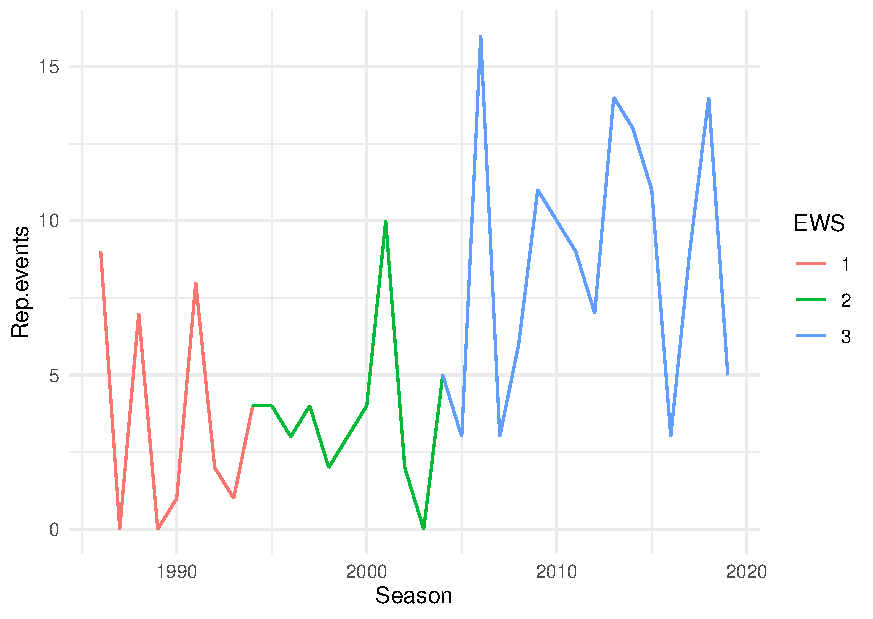
\includegraphics[width = 0.45\textwidth]{../ava_sea}
	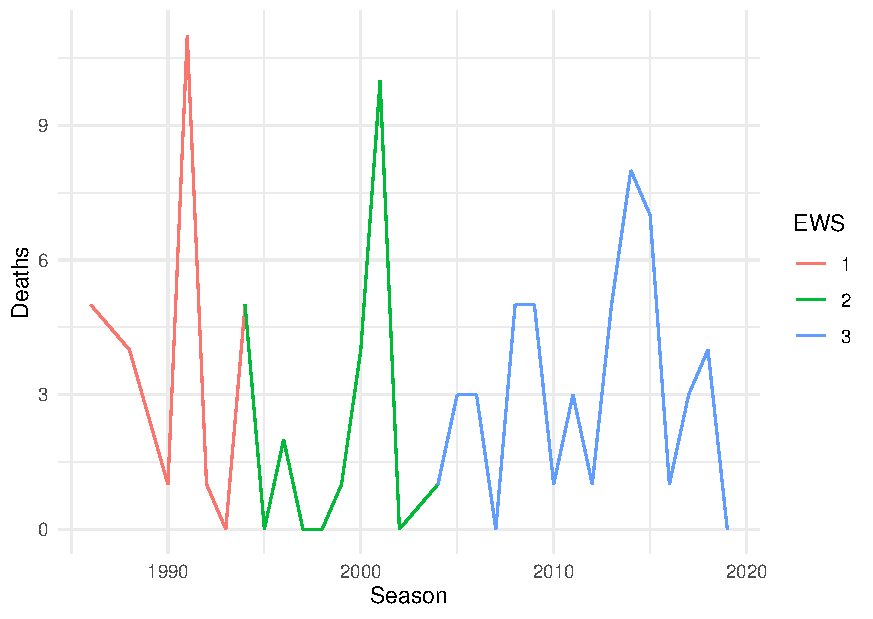
\includegraphics[width = 0.45\textwidth]{../dea_sea}
	\caption{Plots illustrating the temporal evolution of avalanche related statistics. The EWS measure is 1 = No EADS, 2 = EADS present, 3 = EADS online daily.}
	\label{fig:tempevava}
\end{figure}	

	From the above graphs we can see a positive trend in the number of avalanches and year, but no obvious trend in the number of deaths. We calculate the correlations between the number of deaths and the number of avalanches separated into EWS periods. 
	
	We obtain the following correlations (90\% bootstrap intervals)
\begin{table}[H]
	\centering
	\begin{tabular}{ccc}
		\hline
		No EADS & EADS & EADS Online \\
		\hline
		0.807 (0.9325, 0.9986) & 0.875 (0.1890, 0.9728) & 0.602 (0.3842, 0.8147) \\
		\hline
	\end{tabular}
\end{table}
This shows that the events become less correlated after the general public obtained easy access to EADS. It is not likely that the introduction of EADS increased to correlation, so the observed increase in correlation for that period is likely due to noise (10 events in 2001 resulting in 10 deaths). However it may also be due to an increase in user confidence, which led to foolish behaviour.

We are now going to model the number of deaths in avalanches. We are using a Poisson model with a logarithmic (canonical) link function. 

Our formulae are as follows:

\begin{align*}
\lambda_i &= \mathrm{Rep.events}_i \cdot \exp(\beta_0 + \beta_1 \cdot \mathrm{EADS1}_i + \beta_2 \cdot \mathrm{EADS2}_i)\\
\log(\lambda_i) &= \beta_0 + \beta_1 \cdot \mathrm{EADS1}_i + \beta_2 \cdot \mathrm{EADS2}_i) + \ln(\mathrm{Rep.events}_i)\\
\mathrm{Deaths}_i &\sim \mathrm{Poisson}(\lambda_i)
\end{align*}

We note that these parameters have a multiplicative effect on the rate, so it is fine to have an intercept on physical terms. We will remove the intercept later. Note that we are using an offset, as we are calculating the rate of casualty per avalanche, so the rate should be the same per avalanche and hence the offset.

We could model without the offset and with a regression coefficient on the number of avalanches. However this nonsensical, as it would imply that there can be avalanche deaths without an avalanche even occurring. That model also had quite a bit larger DIC (and was overall worse in other measures such as WAIC and LOO) than the model that we are using.

We place wide normal priors on all $\beta_i$ and code up our model. The code is given in \ref{code:stan_1}, with a JAGS version given in \ref{code:jags_1}. 

We run it and obtain the following posterior summaries. We have exponentiated our parameters prior to summarising to ease interpretation.

\begin{table}[ht]
	\centering
	\begin{tabular}{rrrr}
		\hline
		& (Intercept) & EADS1TRUE & EADS2TRUE \\ 
		\hline
		Min. & 0.30 & 0.26 & 0.16 \\ 
		1st Qu. & 0.66 & 0.64 & 0.39 \\ 
		Median & 0.77 & 0.78 & 0.47 \\ 
		Mean & 0.78 & 0.82 & 0.48 \\ 
		3rd Qu. & 0.89 & 0.96 & 0.55 \\ 
		Max. & 1.64 & 2.44 & 1.21 \\ 
		\hline
	\end{tabular}
\caption{Posterior summaries for the first Poisson model}
\label{tab:postsum_po}
\end{table}

From this we can make some initial conclusions. We see that the expected number of deaths per avalanche given no mitigation is 0.78. We also see that each EADS evolution decreases the expected number of deaths, by 0.82 and 0.48 times respectively (if all other variables are held constant). The latter is a rather large decrease, befitting of the drastic change in preparation tact that the EADS going online brought about.

We are interested in the posterior predictive distribution. We want to predict the probability of observing less than 15 deaths given 20 avalanches next year. We know that the EADS will still be online, so we have the appropriate data. 

We obtain a probability of $P(D<15|A=20, EADS=2) = 0.987$.

We are also interested in the probability of observing more than 1 death in mean per avalanche in each stage of the EADS lifespan (not present, present, online). For this we need to calculate $$P\left(\frac{\lambda}{\mathrm{Rep.events}}>1 \ \vline \ \mathrm{EADS}=x\right).$$ Given our offsetting this is rather simple, as this simplifies to $$P\left(\exp(\beta_0 + \beta_1 \cdot \mathrm{EADS1} + \beta_2 \cdot \mathrm{EADS2}) > 1 | \mathrm{EADS} = x\right),$$
of which we have posterior samples.

We calculate these probabilities for all values of the EADS and obtain
\begin{table}[ht]
	\centering
\begin{tabular}{ccc}
	\hline
	No EADS & EADS & EADS online \\
	\hline
	0.104 & 0.005 & 0 \\
	\hline
\end{tabular}
\caption{Probabilities of multiple fatalities per avalanche given the various states of the EADS}
\label{tab:probmdpa}
\end{table}

After this we are told that on average the number of avalanches per year is between 5 and 15, and that they consider that for an extreme number of events that the number of casualties could be 4 times greater (or lesser) than the average number of casualties. 

From this we work out that the mean number of avalanches is 10 with standard deviation 5. We also want to give the multiplier high mass between 0.25 and 4. 

Suggested is a log-normal prior with mean 0 and standard deviation 2 on \[\phi = \exp((x-\mu_x)\cdot\beta_{\mathrm{Rep.events}}),\] the multiplier. This implies a normal prior with mean 0 and standard deviation 2 for $(x-\mu_x)\cdot\beta_{\mathrm{Rep.events}}$, or $\beta_{\mathrm{Rep.events}} \sim N(\mu = 0, \sigma^2 = 4(x-\mu_x)^2).$ There could be problems with this, as it is possible for $(x-\mu_x)$ to be 0. 

The mean and standard deviation parameters for a lognormal distribution are typically given as the mean and standard deviation of the underlying normal distribution. Hence we calculate the true mean and SD as \[\mu_{\phi} = \exp\left(0 + \frac{2^2}{2}\right) = e^2 \approx 7.39, \qquad \sigma^2_{\phi} = (\exp(2^2)-1)\exp(2\cdot0 + 2^2) = e^8 - e^4 \approx 2925, \implies \sigma \approx 54.\] This is clearly not appropriate for the multiplier, as the mean is too high, and the standard deviation even moreso.
\printbibliography

\newpage

\appendix

\section{Code for Question 1}
\subsection{R}
%\inputminted{R}{../Q1.R}
\tcbr{../Q1.R}
\label{code:main_1}
\subsection{Stan}
\tcbstan{../stan/poisson_glm.stan}
\tcbstan{../stan/poisson_glm_exvar.stan}
\label{code:stan_1}
\subsection{JAGS}
\tcbr{../jags/Q1jags.R}
\tcbjags{../jags/poisson.jags}
\tcbjags{../jags/poisson_exvar.jags}
\label{code:jags_1}
\section{Code for Question 2}
\subsection{R}
\tcbr{../Q2.R}
\label{code:main_2}
\subsection{Stan}
\tcbstan{../stan/binomial_glm.stan}
\tcbstan{../stan/binomial_glm_randomeffects.stan}
\label{code:stan_2}
\end{document}

